%----------------------------------------------------------------------------------------
%	PACKAGES AND OTHER DOCUMENT CONFIGURATIONS
%----------------------------------------------------------------------------------------
\documentclass[a4paper,11pt]{article}
\usepackage[a4paper,textwidth=140mm,textheight=245mm]{geometry}
\usepackage[utf8]{inputenc}
\usepackage{listings}
\usepackage{graphicx}
\usepackage{mathtools}
\usepackage{subscript}
\usepackage{tikz}
\usepackage{float}
\makeatletter
\renewcommand{\section}{\@startsection
   {section}%                         name
   {1}%                               level
   {0mm}%                             indent
   {-1.5\baselineskip}%               space above header
   {0.5\baselineskip}%                space under header
   {\sffamily\bfseries\upshape\normalsize}}% style
\renewcommand{\subsection}{\@startsection
   {subsection}%                      name
   {2}%                               level
   {0mm}%                             indent
   {-0.75\baselineskip}%              space above header
   {0.25\baselineskip}%               space under header
   {\rmfamily\normalfont\slshape\normalsize}}% style
\renewcommand{\subsubsection}{\@startsection
   {subsubsection}%                    name
   {3}%                               level
   {-10mm}%                             indent
   {-0.75\baselineskip}%              space above header
   {0.25\baselineskip}%               space under header
   {\rmfamily\normalfont\slshape\normalsize}}% style
\makeatother
\begin{document}

\begin{titlepage}
\title{TSIT03 Summary:}
\author{Martin Söderén\\ marso329@student.liu.se\\900929-1098}
\date{\today}
\maketitle
\vfill % Fill the rest of the page with whitespace
\thispagestyle{empty}
\end{titlepage}
\section{Ceaser cipher}
\subsection{Overall information}
25 possible keys(ENG). You shift the alphabet n times so with key 1 or b(what a becomes) "a" becomes "b" and so on.
\subsection{Cryptoanalysis}
\begin{itemize}
\item Long texts with no plaintext: Break by looking at the distribution of letters. 
\item Short texts with known plaintext: Count number of occurences of each letter and match.
\item Short text with no plaintext: Test each key
\end{itemize}

\section{Simple substitution cipher}
\subsection{Overall information}
$26!$ number of keys. A substitution alphabet is created somehow by mostly a keyword and this tells which letter is substituded for which letter.
\subsection{Cryptoanalysis}
Use the freqency distribution to find a suitable match. 
\section{Vigenere Cipher}
\subsection{Overall information}
Changes subsitution for each position. 
\subsection{cryptoanalysis}
Guess the key length and solve the responding ceasar cipher.

\section{Block cipher}

\subsection{Criteria}
confusion(non-linearity) and Diffusion(one bit change in input should change several characters of the output).
\newline
\newline 
Strict avalanche criterion:(diffusion) ays that a change in one bit in the input
should change each output bit with probability 1/2.
\subsection{Choose IV}
Choose a random number and send it to the receiver. 

\subsection{Differential cryptanalysis}
It is the study of how differences in information input can affect the resultant difference at the output.

\subsection{partial/statistical linearity}
Can be used to analyze block ciphers and break them.

\subsection{Electronic codebook mode}
Each block is encrypted using a symmetric key and no permutation is used between the blocks. The means that two identical blocks are encrypted into the same cryptotext. This is pretty clear when encrypting a .bmp image. Does not require a IV.

\subsection{Cipher block chaining mode} 
Each blocks plaintext is XOR:ed with the previous blocks cryptotext. To make each messadce unique a initialization vector is used. Gives integrity.
\begin{figure}[H]
  \centering
  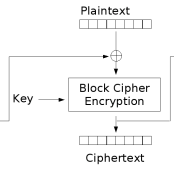
\includegraphics[scale=0.6]{cbc.png}
  \caption{Cipher block chaining}
\end{figure}


\subsection{Propagating Cipher Block Chaining}
As cipher block chaining but the plaintext is XOR:ed with the previous block plaintext and ciphertext. 

\subsection{Cipher Feedback mode}
Works as a self-synchronizing stream cipher. Gives integrity.

\subsection{Output Feedback}
synchronous stream cipher. Can run in parallell. Runs as a stream cipher, no message integrity check
\begin{figure}[H]
  \centering
  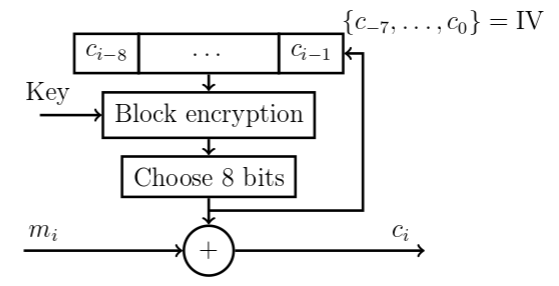
\includegraphics[scale=0.4]{ofm.png}
  \caption{Output feedback mode}
\end{figure}
\subsection{Counter mode}
Turns block cipher into stream cipher and uses a counter to make each block unique. 

\subsection{Authenticated Encryption mode}
A mac is sent that is either generated on the plaintext och the ciphertext. 




\section{DES}
\subsection{Overall information}
Fast in hardware. 64 bit key with 56 effective length. 16 rounds in the feistel network. 64 bit blocks.
\begin{figure}[H]
  \centering
  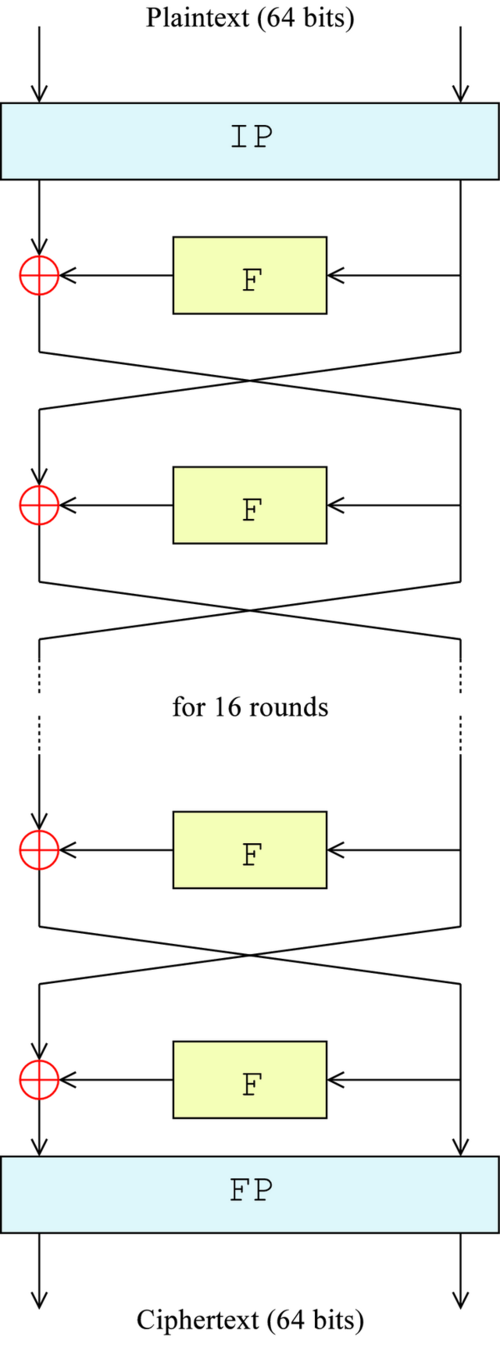
\includegraphics[scale=0.2]{des.png}
  \caption{DES feistel network}
\end{figure}
\subsection{Cryptoanalysis}
Exhaustive search
\subsection{2DES/double des}
$2^{57}$ keys compared to $2^{56} $ in regular DES because of the meet-in-the-middle attack. You need to know the plaintext and the cryptotext. You encrypt the plaintext with all possible encryotions and and decrypt the cryptotext with all possible decryptions and search for a match between those two.
\subsection{3DES}
112 bits of security.

\section{Diffie-Hellman}
Used to exchange keys on public channels. 
\subsection{Explanation using colors}
Red is a private color. Bob has blue and Alice has green. Bob mixes his blue with public red and Alice mixes green with the public red. They exchange them and mix them with their own private color. They now share white. In reality this is used by using big numbers and the problem that it uses is the discrete logarithm problem. 
\subsection{vulnerabilities}
Man-in-the-middle attack. You need twice as many bits as you want the bits of security to be. Much shorter than RSA however.
\subsection{Autentication}
Station-to-station protocol or trust network.

\section{Wide-mouthed-frog protocol}
Autentication through secure server. Each part has a key to the server and the part the starts the communcation sends a key to the second part through the server.
\subsection{vulnerabilities}
Requires global clock, the server knows all the keys, the first part generates the key and needs to be competent to generate a good one.

\section{Hash function}
practiclly impossible to invert. Should be collision free, hash(m1)=hash(m2) with m1!=m2 should not exists. Today the standard is SHA-3 (Keccak)
\subsection{Iterative hash functions}
Hashes arbitrary sized data with a hash function that takes fixed size. Hash functions are pipelined.
\subsection{What to look for in a hash function}
pre-image resistance given a value h it should be difficult to find a m so that h=hash(m) just like a one-way function.
\newline
\newline
second pre-image resistance: Given $m_1$ it should be difficult to find a $m_2$ so that 
$hash(m_1)=hash(m_2)$
\newline
\newline
ollision resistance:It should be difficult to find two messages so that $hash(m_1)=hash(m_2)$. So you can make a person sign one thing and then change it for another.

\subsection{Birthday attack}
You create one good contract m and a fraudulant contract m'. Then finds places in m which can be changed and finds places in m' which can be changed then tries all combinations until m and m' gives the same hash value.
Then make a person sign m och change m for m'. If you find 30 things than can be changed in a document this gives $2^{30}$ different documents. If the hash value is less than 60 bits the probability for a match is large.
\newline
\newline
To prevent this attack the hash function needs to output a value twice as many bits that are needed to prevent a brute-force-attack.

\section{Elliptic curve cryptography}
Same security with shorter keys as other systems.
The matematical problem is based on elliptic curve discrete logarithm problem which means that id you have two point A and B on a elliptic curve is it hard to find a k so A=k*B. An elliptic curve is described by: $$y^2=x^3+ax+b$$

\subsection{How it is used}
The public key is a curve $E \ mod \ p$ where p is a prime, a point $\alpha$ on this curve and a second point $\beta=k*\alpha$ where k is the decryptionkey. To send a secret message to the creator you calculate $(e*\alpha,e*\beta+m)$ where e is a random number and m is the message. The creater decrypt using $$-a(\alpha e)+(e\beta+m)=m$$

\subsection{create a message}
The message m must fulfill $m^3+bm+c$ is a square mod p.

\section{RSA}
\subsection{vulnerabilities}
Index calculus algortihm. Use probability to solve discrete logarithm problems. You need 3248 bits key to get 128 bit bits of security which will makeit secure for the next 30 years.	
\newline
\newline
Bad random generators can cause two n to share factors. If this is the case then $gcd(n_1,n_2)$ is the common factor and you can factor both $n_1$ and $n_2$
\newline
\newline
If the same same n is used in two transmissions with the same message but e and d is different then the message kan be calculated. Example:
receives: $ c_A=m^{e_A} \ mod \ n $ and $c_B=m^{e_B} \ mod \ n$ calculate :$c_A^ac_B^b=m^{ae_A+be_B} \ mod \ n=m$ for some a and b.
\newline
\newline
p and q must be chosen at complete random.
\subsection{Select values}
\begin{enumerate}
\item Select two large primes p and q
\item compute n=pq
\item Choose a value e so that $1<e<(p-1)(q-1)$ and $gcd(e,n)=1$
\item compute a value d so that $d*e \ mod \ (p-1)(q-1)=1  $
\item public key is (e,n) and private key is (d,n)
\end{enumerate}
\subsection{encryption}
m=message
$m^e \ mod \ n=c$

\subsection{decryption}
$m=c^d \ mod \ n$


\section{ElGamal}
\subsection{Public key}
\begin{enumerate}
\item Choose a great prime p
\item choose a number g between 1 and p-1
\item select a random number x to be private key
\item calculate $y=g^x mod \ p$
\item the public key is p,g,y and the private key is x.
\end{enumerate}

\subsection{Encryption}
\begin{enumerate}
\item message to send is m
\item select a random number k
\item calculate $a=g^k\ mod \ p$
\item calulcate $b=y^km \ mod \ p$
\item send \textit{a} and \textit{b}
\end{enumerate}

\subsection{Decryption}
$m=\dfrac{b}{a^x}\ mod \ p$

\subsection{vulernabilites}
If you reuse k the a value will be the same so a easedropper will notice this. This means that the attacker can calculate $\dfrac{m_1}{m_2}$ if message statistics are known. 

\section{Electronic cash}
\subsection{Requirements}
\begin{itemize}
\item Secure transfer in computer networks
\item Cannot be copied and reused
\item Anonymity
\item Offine transactions
\item Can be transferred to others
\item Can be subdivided
\end{itemize}

\subsection{Protocols}
blind signatures and secret sharing

\section{Quantum key distribution}
\subsection{Steps}
\begin{enumerate}
\item Key exchange
\item key sifting
\item error correction
\item privacy amplification
\item authentication
\end{enumerate}
\subsection{Encoding}
The most common encoding is into singlo photon polarization. 0/1 is encoding into vertical/horizontal polarization or +- 45 degrees polarization. The polarization must be chosen at random.

\subsection{Easedropper}
If the noise on the channel is to great there is a big chance that there is a easedropper on the channel since listening on the channel will increase the noise since you cannot read the polarization of the photon without changing it(Heisenberg). BB84 can handle up to 11 procent of noise.

\section{One time pad}
\subsection{Requirements}
The key can never be reused. Key needs to be truly random. The key needs to be the same length as the message. The key needs to remain secret.

\subsection{Relation with stream cipher}
In stream cipher a pseudo random keystream is generated from a shorter key to mimic a one time pad. 

\section{Stream cipher}
\subsection{Types}
Synchronous stream ciphers: The keystream is generated completely independent from the ciphertext.
\newline
\newline
Self-synchronizing stream ciphers: The keystream is generated using the ciphertext which can make it possible to recover from errors on the channel.

\section{AES}
Does not use Feistel. 128 bit block size, recommended key is 128 but 192 and 256 is available.
\subsection{Encryption}
\begin{enumerate}
\item Keyexpansion. The key is expanded so each round gets a 128 bit key.
\item Initialround - each byte of the state is combined with a block of the round key using bitwise xor.
\item rounds 
\begin{enumerate}
\item SubBytes - Each byte is replaced according to a lookup table (nonlinear, uses $1/x$ function)
\item Shiftrows
\item Mixcolumns
\item Addroundkey
\end{enumerate}
\item Finalround - same as rounds but without mixcolumns
\end{enumerate}
\begin{figure}[H]
  \centering
  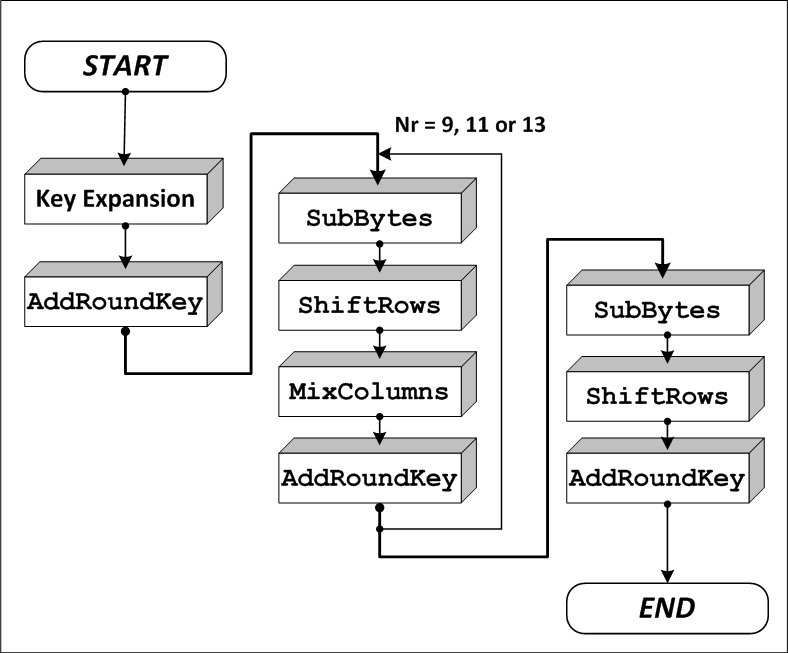
\includegraphics[scale=0.4]{AES.jpg}
  \caption{AES blocks}
\end{figure}

\section{ Linear Feedback Shift Register}
for a lfsr of size n the maximum cycle length is $n^2-1$
\subsection{Vulernabilities}
Ciphers can be broken with  Berlekamp-Massey algorithm. To do this you need 2n bits if a n bit lfsr is used.
\subsection{a5/1}
lfsr is used in the a5/1 cipher for the a2 network. To get around the problem with the Berlekamp-Massey algorithm irregular clocking is used.

\section{zero knowledge}
\subsection{steps}
\begin{enumerate}
\item The prover commits to something that he claims to know. It must be easy for the verifier to verify but hard to calculate.
\item The verifier issus a challenge and the prover responds with a answer.
\item the commitment must be random
\end{enumerate}

\end{document}